\section{Objective}\label{sec:objective}

The primary objective of this project is to build a machine that can effectively compete with a human in foosball.
More specifically, the machine should be able to:

\begin{itemize}
    \item Defend against balls traveling at speeds of up to $7m/s$.
    This is approximately the speed achieved by normal players when they try to shoot fast.
    \item Shoot the ball back with a speed of $7m/s$.
    \item Achieve a positional precision of $0.1mm$, which is circa the accuracy of normal stepper motors (including the mechanics to move the players).
\end{itemize}


\section{Motors}\label{sec:motors}

\subsection{Objectives}\label{subsec:objectives}
I want to be able to defend a ball with a velocity of maximum $v=7m/s$.

\subsection{Table measurements}\label{subsec:table_measurements}
This picture shows the table with the measurements:

\begin{center}

    \begin{tikzpicture}
        \node[anchor=south west,inner sep=0] (image) at (0,0) {\includegraphics[width=0.5\textwidth]{../photos/foosball_table}};
        \begin{scope}
            [x={(image.south east)},y={(image.north west)}]
%        \draw[help lines,xstep=.1,ystep=.1] (0,0) grid (1,1);
%        \foreach \x in {0,1,...,9} { \node [anchor=north] at (\x/10,0) {0.\x}; }
%        \foreach \y in {0,1,...,9} { \node [anchor=east] at (0,\y/10) {0.\y}; }
            \def \tubex {0.76};
%        \draw[red,ultra thick,rounded corners] (0.62,0.65) rectangle (0.78,0.75);
            \draw[<->,blue!80!black!50,rounded corners, line width=1.5mm] (\tubex, 0.9)  -- (\tubex, 0.65) node[midway, left, fill=white, fill opacity=0.8,text opacity=1,rounded corners=2pt,inner sep=1pt] {\huge \textbf{180mm}};
            \draw[<->,blue!80!black!100,rounded corners, line width=1.5mm] (0.85, 0.9)  -- (0.85, 0.09) node[pos=0.85, left, fill=white, fill opacity=0.8,text opacity=1,rounded corners=2pt,inner sep=1pt] {\huge \textbf{700mm}};
            \draw[<->,blue!80!black!70,rounded corners, line width=1.5mm] (0.335, 0.5)  -- (0.775, 0.5) node[pos=0.85, left, fill=white, fill opacity=0.8,text opacity=1,rounded corners=2pt,inner sep=1pt] {\huge \textbf{400mm}};

        \end{scope}
    \end{tikzpicture}
\end{center}
%\todo{The calculations dont make completly sense, i think i made a mistake somewhere and bought an overpowered motor, which is fine i guess}

\subsection{Calculations for the moving motor}\label{subsec:moving_motor}
The distance from the foremost attacker to the goal is $s=0.4m$.
That means the player has to stop the ball in time t, where
\begin{equation}
    \label{eq:stopping_time}
    t = \frac{s}{v} = \frac{0.4m}{7m/s} = 0.057\dots s.
\end{equation}
Which is not a lot of time to process the image and move the motors.
I round the travel distance of the goalkeeper of 180mm to 200mm for the calculations, because there is a spring at the end of the either ends which can be compressed.
I always keep the goalkeeper in the middle, so the player has to travel a maximum distance of 0.1m that means the player has an average velocity of
\begin{equation}
    \label{eq:average_velocity}
    v = \frac{s}{t} = \frac{0.1m}{0.057s} = 1.75m/s.
\end{equation}
I assume a linear acceleration and deceleration, and when the player reaches the top speed it needs to decelerate immediately, so the acceleration and deceleration and therefore the force is as small as possible.
A graph to explain the velocity can be seen here:

\begin{center}
    \begin{tikzpicture}
        \centering
        \begin{axis}
            [
            axis x line=center,
            axis y line=center,
            width={0.2\linewidth},
            xtick=none,
            ytick={0,1},
            yticklabels={,$v_{max}$},
            xlabel={$t$},
            ylabel={$v$},
            xlabel style={below right},
            ylabel style={above left},
            xmin=-0.2,
            xmax=2.2,
            ymin=-0.2,
            ymax=1.2]

            \addplot [] table {
                0 0
                1 1
                2 0
            };
        \end{axis}
    \end{tikzpicture}
\end{center}

\noindent Which means the player has a top speed of at least $2\cdot1.75m/s=3.5m/s$, as the motors have to accelerate and decelerate.
The motor also needs to be able to accelerate the player in $0.057s/2=0.0285$, which means the motor needs to be able to achieve a maximum acceleration $a$ of
\begin{equation}
    \label{eq:acceleration}
    a = \frac{v}{t} = \frac{3.5m/s}{0.0285s} = 122.8m/s^2.
\end{equation}
I assume that the weight of the tubes is $m \approx 0.1kg$.
The torque needed to move the tubes is
\begin{equation}
    \label{eq:torque}
    \tau = F \cdot r = m \cdot a \cdot r = 0.1kg \cdot 122.8m/s^2 \cdot 0.083m \approx 1Nm
\end{equation}
assuming the radius $r_g$ of the gear is 8.3cm.
And the required top rotational speed (measured in rotations per minute $\text{RPM}$) is
\begin{equation}
    \label{eq:top_rpm}
    \frac{v}{2\pi r_g} \cdot 60s/min = \frac{7m/s}{2\pi \cdot 0.083m} \cdot 60s/min \approx 800\text{RPM}.
\end{equation}
A Motor that fits those requirements is the \textbf{PD42-3-1141\autocite{PD42-3-1141}} from \textbf{Trinamic}.

\subsection{Calculations for the rotating motor}\label{subsec:rotating_motor}
The ball has a mass $m=17g$.
I assume that I have an angle of $45\deg$ ($=\frac{\pi}{4}$ in radians) to accelerate the ball.
\\
\begin{center}

    \tikzset{
        testpic/.pic={
            \node at (0.05,-0.35) {
\includegraphics[height=3.2cm] {../photos/foosball_player}};
        },
        testpic2/.pic={
            \node at (0.05,-0.35) {
\includegraphics[height=3.2cm] {../photos/foosball_player}};
        },
    }

    \begin{tikzpicture}
        \def \r {2cm}
        \def \rsmall {0.5}
        \def \angle {45}
        \pic[rotate=45/2,transform shape] at (0,0) {testpic};
        \pic[rotate=-45/2,transform shape] at (0,0) {testpic2};
        \draw (0,0) -- ({-sin(\angle / 2)*\r}, {-cos(\angle / 2)*\r});
        \draw (0,0) -- ({sin(\angle / 2)*\r}, {-cos(\angle / 2)*\r}) node[right, midway] {$r_p=70\text{mm}$};
        \draw ({-sin(\angle / 2)*\rsmall}, {-cos(\angle / 2)*\rsmall}) arc(270-\angle/2:270+\angle/2:\rsmall) node[midway,below] {$45\deg$};
        \draw[->] ({-sin(\angle / 2)*\r}, {-cos(\angle / 2)*\r}) arc(270-\angle/2:270+\angle/2:\r) node[midway,below] {$l$};
%        \draw () circle (\r);
    \end{tikzpicture}
\end{center}
%    \\
That means the player has the distance $l$ to accelerate the ball together with the player.
\begin{equation}
    \label{eq:distance}
    l = r_p \cdot \frac{\pi}{4} = 70mm \cdot \frac{\pi}{4} = 55mm
\end{equation}
The goal is to shoot the ball back at a speed of 7m/s.
The time to accelerate the ball is
\begin{equation}
    \label{eq:time}
    t = \frac{2\pi\cdot r_p}{v} = \frac{2\pi\cdot 70mm}{7m/s} = \frac{\pi}{50} \approx 0.06s
\end{equation}
The maximum speed can easily be calculated with
\begin{equation}
    \label{eq:max_speed}
    \omega = \frac{60s/min}{t} = \frac{60s/min}{0.6s/rotation} = 1000\text{RPM}
\end{equation}
\todo{Compute the torque needed to accelerate the ball}
For the motor that just rotates the figure I can use a DC motor with gears and an encoder, as they often have more power and can go faster with less torque and accuracy.
% Pololu 10:1 Metal Gearmotor 37Dx65L mm 12V with 64 CPR Encoder (Helical Pinion) 4758
A motor that fits those requirements is the \textbf{Pololu 10:1 Metal Gearmotor 37Dx65L mm 12V with 64 CPR Encoder (Helical Pinion) 4758}\autocite{pololu-dc}.


\section{Camera}\label{sec:camera}

\subsection{Optics}\label{subsec:lens}
To achieve my goal of defending against balls at speed of up to $7m/s$, I need a camera that can capture the entire table at a framerate of at least 200fps.
I record the table from the bottom to avoid the players and the rods; therefore, I have to replace the floor of the table with a glass plate.
A sensor that achieves this is the \textbf{IMX287 CMOS} sensor from \textbf{Sony}.
This sensor has a width of $4.98\text{mm}$.
Here is a schematic of the approximate setup for the camera:\\
\begin{center}
    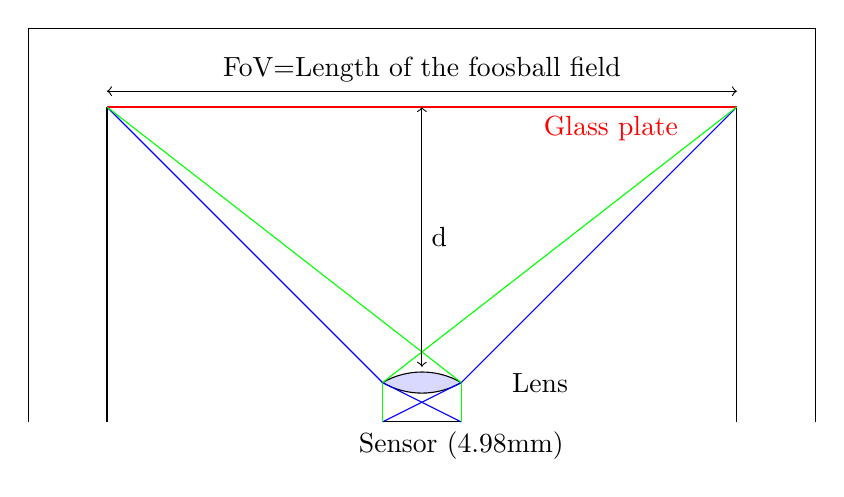
\begin{tikzpicture}
        \draw (0,0) -- (0, 5);
        \draw (0, 5) -- (10, 5);
        \draw (10, 5) -- (10, 0);

        \draw (1,0) -- (1, 4);
        \draw[red] (1, 4) -- (9, 4) node[pos=0.8, below] {Glass plate};
        \draw (9, 4) -- (9, 0);

        \draw (4.5, 0) -- (5.5, 0) node[below] {Sensor (4.98mm)};

        \pgfmathsetmacro{\lensRadius}{1}
        \pgfmathsetmacro{\lensHeight}{0.5}
        \pgfmathsetmacro{\startAngle}{asin(\lensHeight/\lensRadius)}

        \draw [fill=blue!15]  (4.5,\lensHeight)
        arc[start angle=180-\startAngle+90,delta angle=2*\startAngle,radius=\lensRadius]
        arc[start angle=-\startAngle+90,delta angle=2*\startAngle,radius=\lensRadius]
        -- cycle; % to get a better line end

        \draw[blue] (1, 4) -- (4.5, \lensHeight);
        \draw[blue] (4.5, \lensHeight) -- (5.5, 0);

        \draw[blue] (9, 4) -- (5.5, \lensHeight);
        \draw[blue] (5.5, \lensHeight) -- (4.5, 0);

        \draw[green] (1, 4) -- (5.5, \lensHeight);
        \draw[green] (5.5, \lensHeight) -- (5.5, 0);

        \draw[green] (9, 4) -- (4.5, \lensHeight);
        \draw[green] (4.5, \lensHeight) -- (4.5, 0);

        \draw (6.5, 0.5) node[]{Lens};
        \draw[<->] (5, 0.70) -- (5, 4) node[midway, right] {d};
        \draw[<->] (1, 4.2) -- (9, 4.2) node[above, midway] {FoV=Length of the foosball field};
    \end{tikzpicture}
\end{center}

\paragraph{Lens Equation}\label{par:lens_equation}

The relationship between the object width (FoV), sensor width, and distance to the object is given by:
\begin{equation}
    \text{Object Width (FoV)} = \text{Sensor Width} \times \frac{\text{Distance to Object (d)}}{\text{Focal Length (f)}}\label{eq:lens_equation}
\end{equation}


\noindent In my case $d = 700mm$ and my Field of View (FoV) is $1200mm$ as this is the length of the foosball field.
Now I solve for the focal length $f$:
\begin{equation}
    \label{eq:focal_length}
    f = \frac{\text{Sensor Width} \times \text{Distance to Object (d)}}{\text{Object Width (FoV)}} = \frac{4.98\text{mm} \times 700\text{mm}}{1200\text{mm}} \approx 2.9\text{mm}
\end{equation}
% Arducam 2.8-12mm Varifocal C-Mount Lens for Raspberry Pi HQ Camera, with C-CS Adapter
A lens that satisfies these requirements is the \textbf{Arducam 2.8-12mm Varifocal C-Mount Lens for Raspberry Pi HQ Camera, with C-CS Adapter} with a focal length of $2.8-12mm$.